\documentclass{article}

% Paquetes comunes
\usepackage[utf8]{inputenc}
\usepackage[T1]{fontenc}
\usepackage[spanish]{babel}
\usepackage{amsmath, amssymb}
\usepackage{graphicx}
\usepackage{float}
\usepackage{geometry}
\usepackage{hyperref}
\usepackage{fancyhdr}
\usepackage{textcomp}
\usepackage{circuitikz}
% Saltar entre párrafos - sin sangrías
\usepackage{parskip}

% Márgenes
\geometry{a4paper, margin=2.5cm}

% Encabezado y pie de página
\pagestyle{fancy}
\fancyhf{}
\fancyhead[L]{\textbf{Tarea 1} - Tomas Infante}
\fancyhead[R]{IEE2513}
\fancyfoot[C]{\thepage}

\title{Tarea 1}
\author{Tomas Infante}
\date{\today}
\begin{document}
\begin{figure}[H]
    \centering
    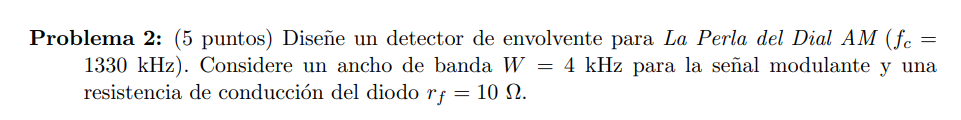
\includegraphics[width=1\textwidth]{Problema_2.png}
    \label{Problema_2}
\end{figure}
Recordemos las condiciones para un buen detector de envolvente:
\begin{enumerate}
    \item Una constane de carga mas rapida que el periodo de de la portadora.
    \item Una constante de descarga mas lenta que el periodo de la portadora, pero mas rapido que el inverso del espectro.
\end{enumerate}
Es decir:
\[
(R_s+r_f)C \ll \frac{1}{f_c} \ll R_L C \ll \frac{1}{W}
\]
Donde circuitalemente el detector de envolvente es:
\begin{figure}[H]
    \centering
    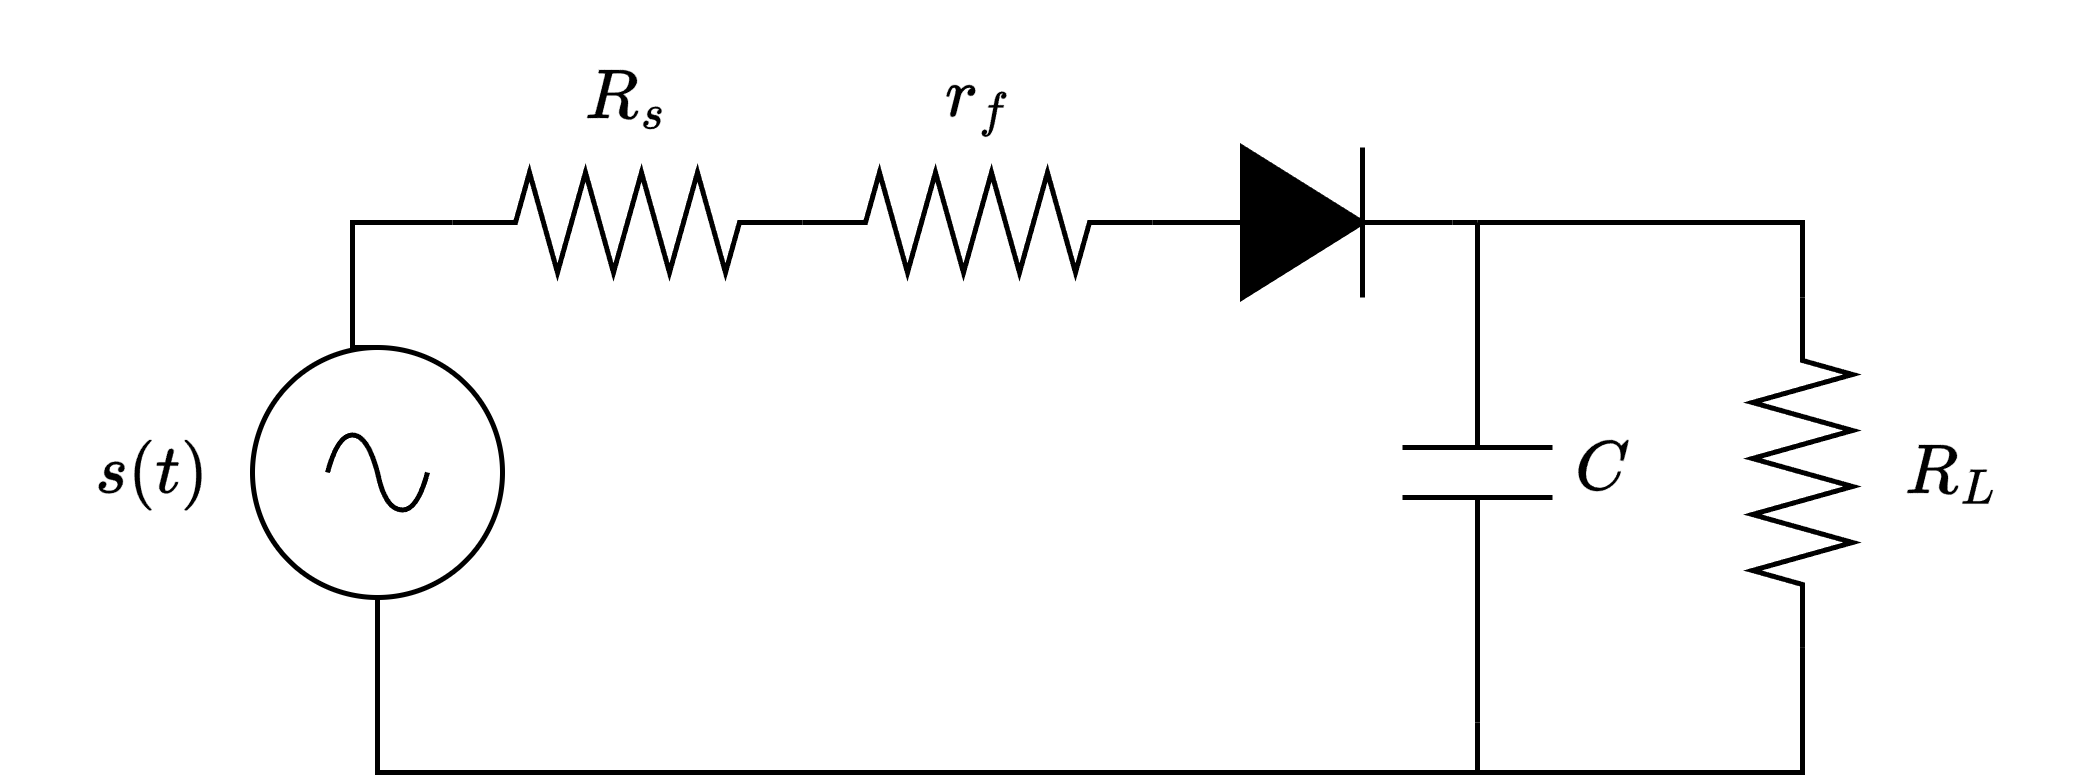
\includegraphics[width=0.6\textwidth]{Detector_Envolvente.png}
    \label{Detector_Envolvente}
\end{figure}
Dado que tenemos el valor de \(f_c = 1330\,\text{kHz}\) y tambien \(W=4\,\text{kHz}\). Podemos encerrar el valor de \(R_{L}C\).
\[
7.519\cdot10^{-7}\ll R_{L}C \ll 2.5\cdot10^{-4}
\]
Si asumimos \(R_s= 50\,\Omega\) y recordamos que \(r_{f} = 10\,\Omega\). Llegamos tambien a la condicion:
\[
(R_s+r_f)C\ll\frac{1}{f_c}\quad \longrightarrow\quad 60 C \ll 7.519\cdot10^{-7}
\]
Es decir:
\[
C \ll 1.253\cdot10^{-8}
\]
Fijamos para dar margen a \(C = 0.5\cdot10^{-8}\,\text{F} = 5\,\text{nF}\). Una vez fijado el valor de \(C\) podemos despejar el de \(R_L\):
\[
\frac{7.519\cdot10^{-7}}{C}\ll R_{L} \ll \frac{2.5\cdot10^{-4}}{C}
\]
\[
\frac{7.519\cdot10^{-7}}{5\cdot10^{-9}}\ll R_{L} \ll \frac{2.5\cdot10^{-4}}{5\cdot10^{-9}}
\]
\[
150.38 \ll R_{L} \ll 50\,\text{k}\Omega
\]
Para dar margen a ambos lados podemos fijar \(R_{L} = 25.1\,\text{k}\Omega\). De esta manera los valores para los componetes circuitales son:
\begin{itemize}
    \item \(C = 5\,\text{nF}\)
    \item \(R_L = 25.1\,\text{k}\Omega\)
\end{itemize}
\begin{figure}[H]
    \centering
    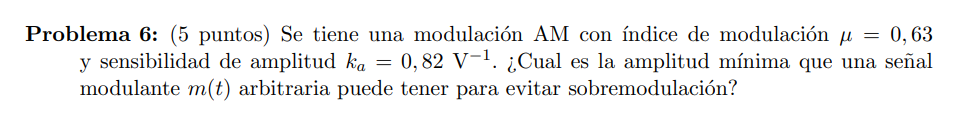
\includegraphics[width=1\textwidth]{Problema_6.png}
    \label{Problema_6}
\end{figure}
Sabemos que:
\[
s(t)=A_c\left[1+k_a m(t)\right]\cos(2\pi f_c t)
\]
Sabemos bien que \(m(t)\) tiene una aplitud minima, es decir donde alcanza su valor minimo, digamos que ese valor es \(A\) (\(A\) eventualemente puede ser negativo). Teniendo en cuenta lo anterior para que no haya sobre modulacion se debe cumplir que:
\[
1+k_aA>0
\]
O equivalentemente, en el peor caso si \(A\) es negativo (Para \(A\) positivo nunca habra sobremodulacion), queremos que se cumpla:
\[
k_a|A|<1 \quad \longrightarrow \quad |A|<\frac{1}{k_a}
\]
Es decir:
\[
|A|<\frac{1}{0.82}=1.219\,\text{V}
\]
\[
|A|<1.219\,\text{V}
\]
Es decir cualquier señal que en algun momento tenga una amplitud de onda que varie hasta los negativos mas alla de los \(-1.219\,\text{V}\) generara sobremodulacion.

\textit{En este contexto se entiende por amplitud minima el valor minimo que alcanza la señal \(m(t)\), es decir, el punto donde la señal toma su valor mas negativo. Dado que el enunciado indica que \(m(t)\) es arbitraria, no se puede asumir que la señal sea simetrica respecto de cero. Por lo tanto, el hecho de que el valor minimo sea \(-A\) no implica necesariamente que la señal alcance el valor \(+A\). Sin embargo, \(|A|\) representa la magnitud de la desviacion minima de la señal hacia valores negativos, que es precisamente el caso relevante para analizar la condicion de no sobremodulacion.}
\begin{figure}[H]
    \centering
    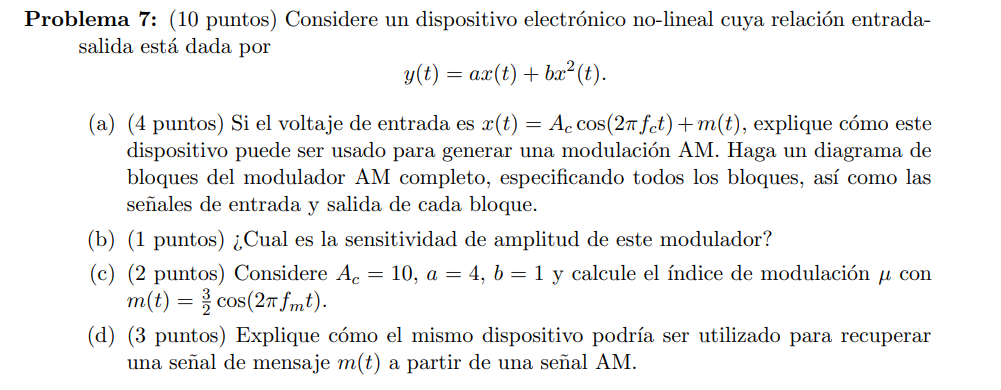
\includegraphics[width=1\textwidth]{Problema_7.png}
    \label{Problema_7}
\end{figure}
\subsection*{a)}
A la entrada \(x(t)\) al ser la entrada del dispositivo este retornarara:
\[
y(t) = a\left[A_c\cos(2\pi f_ct)+m(t)\right]+b\left[A_c\cos(2\pi f_c t)+m(t)\right]^{2}
\]
Donde expandiendo la expresion llegamos a:
\[
y(t)=aA_c\cos(2\pi f_c t)+am(t)+b\left[A_c^{2}\cos(2\pi f_c t)^{2}+2A_c\cos(2\pi f_c t)m(t)+m(t)^{2}\right]
\]
\[
y(t)=aA_c\cos(2\pi f_c t)+am(t)+bA_c^{2}\cos(2\pi f_c t)^{2}+2bA_c\cos(2\pi f_c t)m(t)+bm(t)^{2}
\]
Usamos la propiedad \(\cos(\theta)^{2}=\frac{1+\cos(2\theta)}{2}\).
\[
y(t)=aA_c\cos(2\pi f_c t)+am(t)+bA_c^{2}\left(\frac{1+\cos(4\pi f_c t)}{2}\right)+2bA_c\cos(2\pi f_c t)m(t)+bm(t)^{2}
\]
Factorizamos termino comun \(A_c\cos(2\pi f_c t)\):
\[
y(t) = \left[a+2bm(t)\right]A_c\cos(2\pi f_c t) + am(t)+\frac{bA_c^2}{2}+\frac{bA_c^2}{2}\cos(4\pi f_c t) + bm(t)^2
\]
Aca hay varios terminos interesantes:
\[
y(t) = \underbrace{\left[1+\frac{2b}{a}m(t)\right]\frac{A_c}{a}\cos(2\pi f_c t)}_{\text{Modlacion AM}} +\underbrace{\frac{bA_c^2}{2}}_{\text{DC a eliminar}}+\underbrace{\frac{bA_c^2}{2}\cos(4\pi f_c t) + bm(t)^2 + am(t)}_{\text{AC a eliminar}}
\]
De esta manera podemos asegurar una modulacion AM de la señal \(m(t)\) con nuestro dispositivo no-lineal solo si conseguimos eliminar todo menos la componente que esta acomparañada por \(\cos(2\pi f_c t)\), es decir,
con un filtro pasabanda centrado en \(f_c\) y con ancho de banda \(2W\), donde \(W\) es el ancho de banda de \(m(t)\), lograriamos modular perfectamente. Y obtener:
\[
s(t) = \left[1+\frac{2b}{a}m(t)\right]\frac{A_c}{a}\cos(2\pi f_c t)
\]
En bloques seria:
\begin{figure}[H]
    \centering
    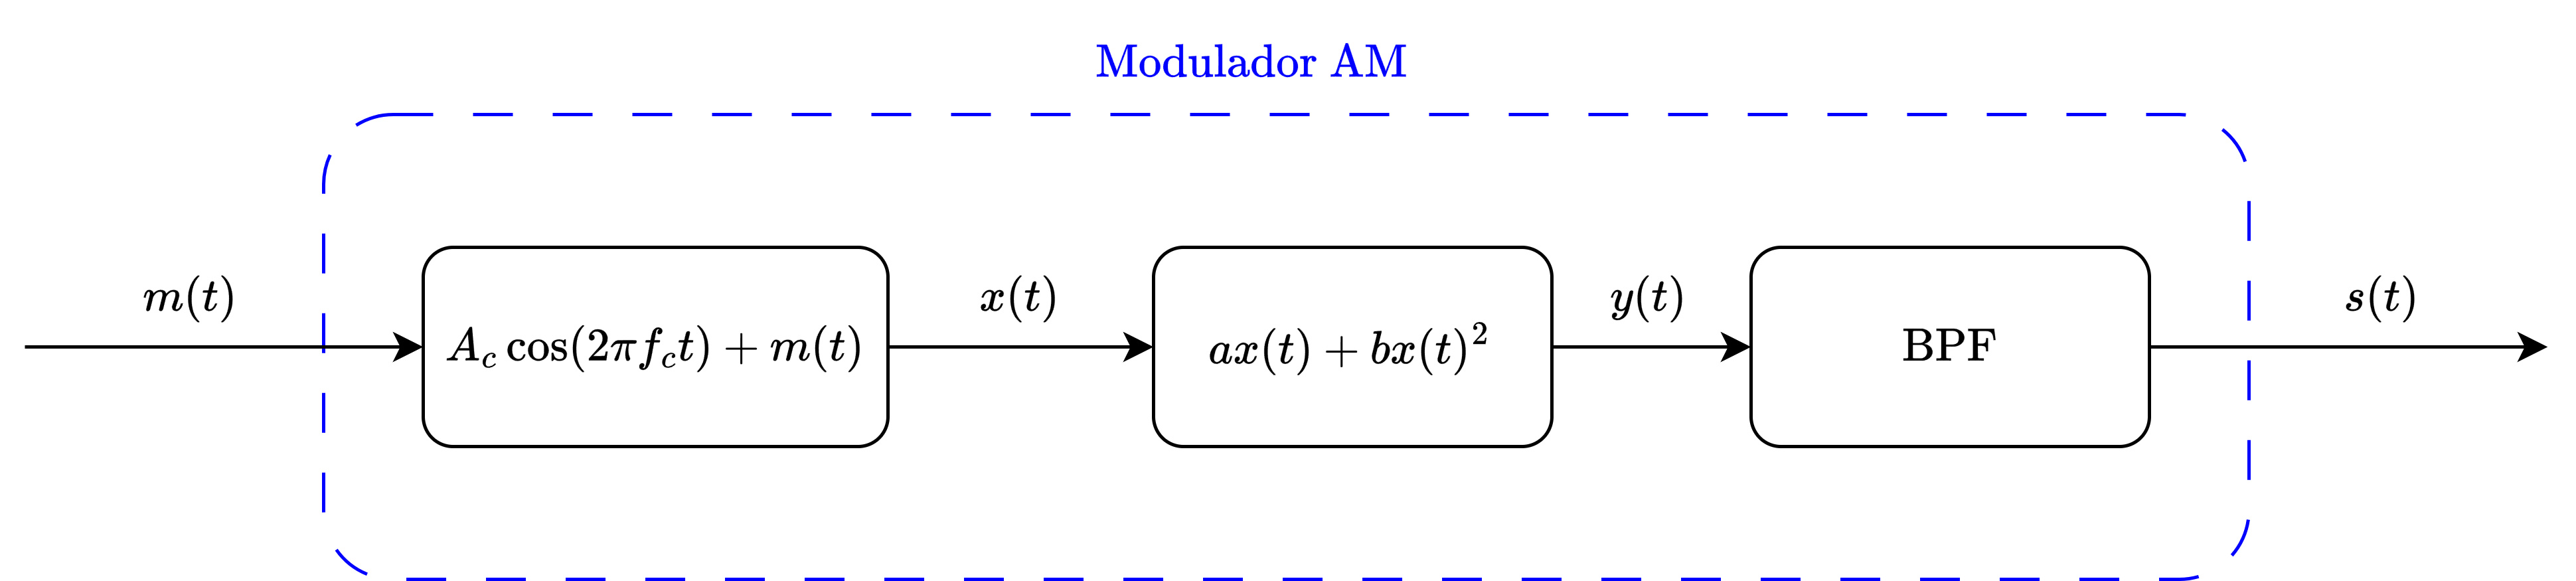
\includegraphics[width=0.9\textwidth]{Diagrama_Bloques.png}
    \label{Diagrama_Bloques}
\end{figure}
Donde la entrada del sistema es la señal que queremos modular \(m(t)\) y la salida \(s(t)\) es la señal moudulada sobre una portadora de frecuencia \(f_c\).
\subsection*{b)}
Recordemos la forma general de una modulacion AM:
\[
s(t) = \left[1+k_am(t)\right]A\cos(2\pi f_c t)
\]
Donde la sensibilidad es \(k_a\) lo que en nuestra expresion:
\[
k_a = \frac{2b}{a}
\]
\subsection*{c)}
Recordemos que el indice de modulacion es \(k_aA_m\) donde \(A_m\) es la amplitud de la señal modulada. En nuestro caso:
\[
m(t)= \frac{3}{2}\cos(2\pi f_m t)
\]
Por lo tanto \(A_m = \frac{3}{2}\) lo cual implica que:
\[
\mu = \frac{3}{2}k_a = \frac{3}{2}\left(\frac{2b}{a}\right)
\]
Si tomamos los valores \(a= 4\) y \(b= 1\). Llegamos a:
\[
\mu = \frac{3}{2}\left(\frac{2}{4}\right) = 0.75
\]
\subsection*{d)}
Usar ese dispositivo para detectar la señal seria equivalente a que la entrada \(x(t)\) del dispositivo sea \(s(t)\) donde:
\[
s(t) = \left[1+\frac{2b}{a}m(t)\right]\frac{A_c}{a}\cos(2\pi f_c t)
\]
Nos quedaria entonces que:
\[
y(t)= a s(t)+b s(t)^{2}
\]
Reemplzamos:
\[
y(t)= \underbrace{a\left[1+\frac{2b}{a}m(t)\right]\frac{A_c}{a}\cos(2\pi f_c t)}_{\text{Factor 1}} + \underbrace{b\left[1+\frac{2b}{a}m(t)\right]^2\left(\frac{A_c}{a}\right)^2\cos^2(2\pi f_c t)}_{\text{Factor 2}}
\]
Podemos notar practicamente por inspeccion que desde el factor 1 es imposible despejar \(m(t)\) asi que solo queda la opcion de evaluar el factor 2. Lo exapandimos.
\[
b\left(\frac{A_c}{a}\right)^2\left[1+\frac{4b}{a}m(t)+\left(\frac{2b}{a}m(t)\right)^2\right]\left[\frac{1+\cos(4\pi f_c t)}{2}\right]
\]
Expandimos un poco:
\[
\frac{b}{2}\left(\frac{A_c}{a}\right)^2\left[1+\frac{4b}{a}m(t)+\left(\frac{2b}{a}m(t)\right)^2\right]+\underbrace{b\left(\frac{A_c}{a}\right)^2\left[1+\frac{4b}{a}m(t)+\left(\frac{2b}{a}m(t)\right)^2\right]\left(\frac{\cos(4\pi f_c t)}{2}\right)}_{\text{No recuperable}}
\]
Toda la expresion señalda es inutil para la recuperacion ya que hay un factor \(\cos(4\pi f_c t)\) que multiplica cada elemento entonces no se podria recuperar \(m(t)\) a diferncia del resto donde si lo expandimos llegamos a:
\[
\underbrace{\frac{b}{2}\left(\frac{A_c}{a}\right)^2}_{\text{DC}}+ \underbrace{\frac{b}{2}\left(\frac{A_c}{a}\right)^2\frac{4b}{a}m(t)}_{\text{Multiplo de }m(t)}+\underbrace{\frac{b}{2}\left(\frac{A_c}{a}\right)^2\left(\frac{2b}{a}m(t)\right)^2}_{\text{AC que deseamos eliminar}}
\]
Finalmente como hay un monomio que es puramente \(m(t)\) por una constante. Llegamos a que se puede recueperar \(m(t)\) solo que habria que aplicar un filtro que logre eliminar todo lo que fuimos eliminando en el camino. Y ademas luego de flitrar seria necesario amplificarlo o atenuarlo dependiendo de si la expresion:
\[
\frac{b}{2}\left(\frac{A_c}{a}\right)^2\frac{4b}{a}
\]
Es mayor o menor a cero. 

Una manera de ver el sistema de recuperacion seria:
\begin{enumerate}
    \item Filtro notch en \(f_c\) para eliminar todo el factor que multiplica a \(\cos(2\pi f_c t)\).
    \item Filtro notch en \(2f_c\) para eliminar todo el factor que multiplica a \(\cos(4\pi f_c t)\).
    \item Filtro pasabanda que elimine DC y la frecuencia fundamental asosiada a \(m(t)^2\).
    \item Amplificador con razon de aplificacion \(\frac{2}{b}\left(\frac{a}{A_c}\right)^2\frac{a}{4b}\).
\end{enumerate}
O tambien una manera mas sencilla seria hacer un filtro pasa bajo dado que eso elimina directamente las frecuencias \(f_c\) y \(2f_c\) ademas como \(f_m \ll f_c\) sobreviviria \(m(t)\). Y luego es necesario pasar al paso 3 y luego al 4.
\begin{figure}[H]
    \centering
    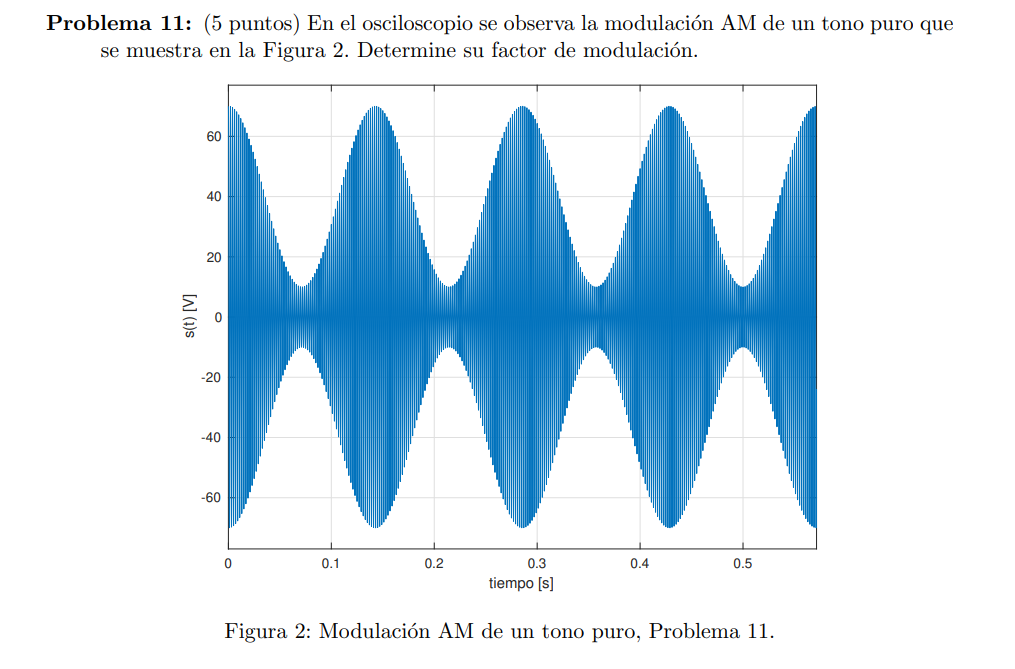
\includegraphics[width=0.9\textwidth]{Problema_11.png}
    \label{Problema_11}
\end{figure}
Sabemos que:
\[
\mu = \frac{A_{\text{MAX}}-A_{\text{MIN}}}{A_{\text{MAX}}+A_{\text{MIN}}}
\]
A partir del grafico podemos, por inspeccion ver que:
\[
A_{\text{MAX}} = 50\,\text{V}\quad A_{\text{MIN}}= 10\,\text{V} 
\]
Por lo tanto:
\[
\mu = \frac{50-10}{50+10} = 0.66
\]
\begin{figure}[H]
    \centering
    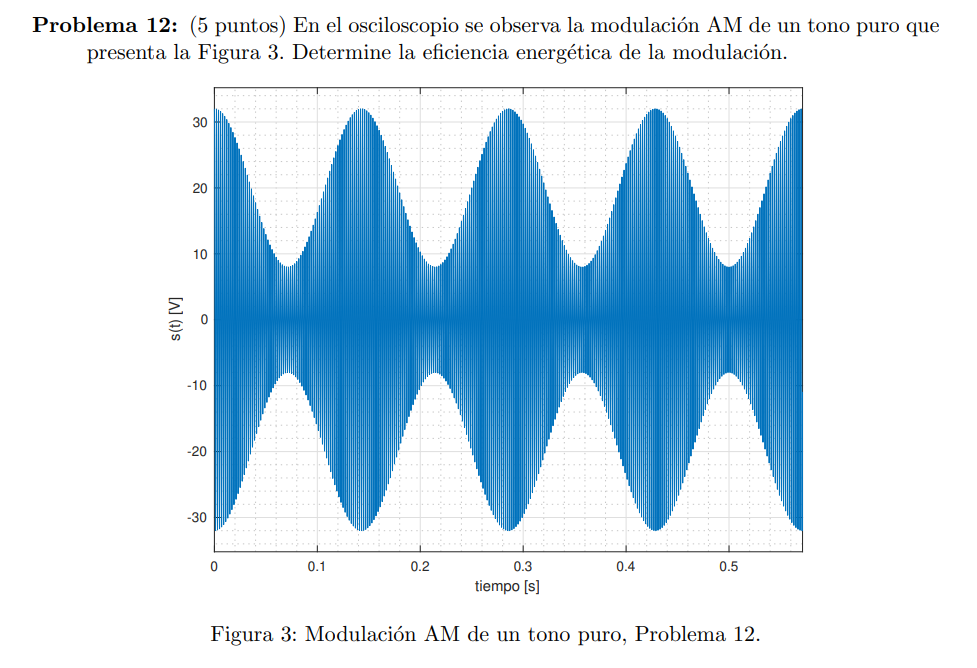
\includegraphics[width=0.9\textwidth]{Problema_12.png}
    \label{Problema_12}
\end{figure}
Sabemos que la ecuacion de eficiencia energetica es:
\[
\eta _{E} = \frac{\mu^{2}}{2+\mu^{2}}
\]
En tal caso primero debemos encontrar \(\mu\), que bien sabemos por el problema 11 es:
\[
\mu = \frac{A_{\text{MAX}}-A_{\text{MIN}}}{A_{\text{MAX}}+A_{\text{MIN}}}
\]
A partir del grafico obtenemos por inspeccion que:
\[
A_{\text{MAX}} = 32\,\text{V}\quad A_{\text{MIN}}= 8\,\text{V} 
\]
Por lo tanto:
\[
\mu = \frac{32-8}{32+8} = 0.6
\]
Se sigue entonces que la eficiencia energetica seria:
\[
\eta _{E} = \frac{(0.6)^{2}}{2+(0.6)^{2}}= 0.1525 = 15,25\%
\]
\end{document}